\chapter{Théorie de l'optimisation sous contraintes}
\label{chap:constrained-optimization}

\section{Problème général}

On considère le problème d'optimisation sous contraintes suivant :
\begin{equation}
    \min_{x \in \mathbb{R}^n} f(x) \quad \text{sous les contraintes} \quad
    \begin{cases}
        c_i(x) = 0, & i \in \mathcal{E}, \\
        c_i(x) \geq 0, & i \in \mathcal{I},
    \end{cases}
\end{equation}
où $f$ et les $c_i$ sont des fonctions régulières (\textit{smooth}), et $\mathcal{E}$ et $\mathcal{I}$ sont des ensembles finis d'indices.

\begin{itemize}
    \item $f$ : fonction objectif (\textit{objective function}).
    \item $c_i$, $i \in \mathcal{E}$ : contraintes d'égalité (\textit{equality constraints}).
    \item $c_i$, $i \in \mathcal{I}$ : contraintes d'inégalité (\textit{inequality constraints}).
\end{itemize}

\section{Ensemble réalisable}

\begin{definition}[Ensemble réalisable]
L'ensemble réalisable (\textit{feasible set}) est l'ensemble des points qui satisfont toutes les contraintes :
\begin{equation}
    \Omega = \left\{ x \in \mathbb{R}^n \mid c_i(x) = 0, \, i \in \mathcal{E} ; \; c_i(x) \geq 0, \, i \in \mathcal{I} \right\}.
\end{equation}
\end{definition}

Le problème peut alors s'écrire de manière équivalente :
\begin{equation}
    \min_{x \in \Omega} f(x).
\end{equation}

Dans ce chapitre, nous étudierons les conditions d'optimalité nécessaires et suffisantes pour ce problème.

\section{Solutions locales}

\begin{definition}[Solution locale]
Un vecteur $x^* \in \mathbb{R}^n$ est une \textbf{solution locale} si :
\begin{enumerate}
    \item $x^* \in \Omega$, et
    \item il existe un voisinage $\mathcal{N}$ de $x^*$ tel que :
    \begin{equation}
        f(x) \geq f(x^*) \quad \text{pour tout } x \in \mathcal{N} \cap \Omega.
    \end{equation}
\end{enumerate}
\end{definition}

\begin{definition}[Solution locale stricte]
Un vecteur $x^*$ est une \textbf{solution locale stricte} si :
\begin{enumerate}
    \item $x^* \in \Omega$, et
    \item il existe un voisinage $\mathcal{N}$ de $x^*$ tel que :
    \begin{equation}
        f(x) > f(x^*) \quad \text{pour tout } x \in \mathcal{N} \cap \Omega, \; x \neq x^*.
    \end{equation}
\end{enumerate}
\end{definition}

\begin{definition}[Solution locale isolée]
Un vecteur $x^*$ est une \textbf{solution locale isolée} si :
\begin{enumerate}
    \item $x^* \in \Omega$, et
    \item il existe un voisinage $\mathcal{N}$ de $x^*$ tel que $x^*$ soit la seule solution locale dans $\mathcal{N} \cap \Omega$.
\end{enumerate}
\end{definition}

\begin{figure}[H]
\centering
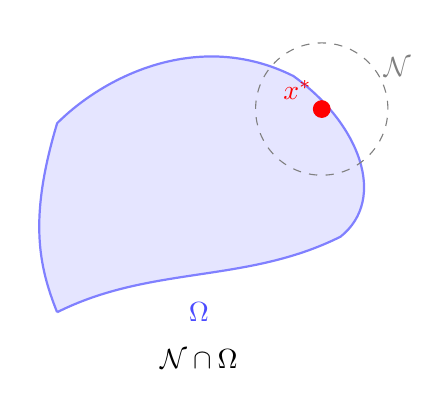
\begin{tikzpicture}[scale=1.2]
    \draw[fill=blue!10, draw=blue!50, thick] (0,0) 
        .. controls (1,0.5) and (2,0.3) .. (3,0.8)
        .. controls (3.5,1.2) and (3.2,2) .. (2.5,2.5)
        .. controls (1.5,3) and (0.5,2.5) .. (0,2)
        .. controls (-0.3,1) and (-0.2,0.5) .. (0,0);
    
    \coordinate (xstar) at (2.8, 2.15);
    \filldraw[red] (xstar) circle (2.5pt) node[above left] {$x^*$};
    
    \draw[dashed, gray] (xstar) circle (0.7cm);
    \node[gray] at (3.6, 2.6) {$\mathcal{N}$};
    
    \node[blue!70] at (1.5, 0.0) {$\Omega$};
    
    \node at (1.5, -0.5) {$\mathcal{N} \cap \Omega$};
\end{tikzpicture}
\caption{Solution locale $x^*$ sur le bord de $\Omega$ : le voisinage $\mathcal{N}$ n'est pas nécessairement inclus dans $\Omega$.}
\label{fig:local-solution-feasible}
\end{figure}

\section{Rappel : Équivalence problème lisse/non-lisse}

\begin{remarque}
Si $g_1, \dots, g_m$ sont des fonctions scalaires régulières, alors le problème non-lisse et sans contraintes :
\begin{equation}
    \min_{x \in \mathbb{R}^n} \left[ \max_{\mu = 1, \dots, m} g_\mu(x) \right]
\end{equation}
est équivalent au problème lisse et sous contraintes :
\begin{equation}
    \min_{(x, t) \in \mathbb{R}^{n+1}} t \quad \text{sous les contraintes} \quad t - g_\mu(x) \geq 0, \quad \mu = 1, \dots, m.
\end{equation}
\end{remarque}

\begin{figure}[H]
\centering
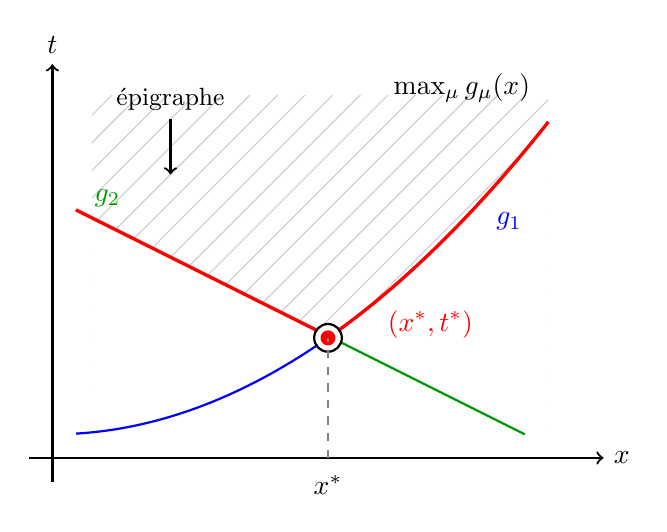
\begin{tikzpicture}[scale=1.0]
    
    % g1 = 0.1*x^2 + 0.3, g2 = -0.5*x + 3.3
    
    \begin{scope}
        \clip (0.5, 0.1) rectangle (6.3, 4.6);
        \foreach \i in {-12,-11,...,25} {
            \draw[gray!40, thin] (\i*0.35, 0) -- (\i*0.35 + 6, 6);
        }
    \end{scope}
    
    \begin{scope}
        \clip (0.5, -0.5) rectangle (3.5, 4.8);
        \fill[white] (0.5, -0.5) 
            -- plot[domain=0.5:3.5, samples=50] (\x, {-0.5*\x + 3.3})
            -- (3.5, -0.5) -- cycle;
    \end{scope}
    
    \begin{scope}
        \clip (3.5, -0.5) rectangle (6.3, 4.8);
        \fill[white] (3.5, -0.5) 
            -- (3.5, {0.1*3.5*3.5 + 0.3})
            -- plot[domain=3.5:6.3, samples=50] (\x, {0.1*\x*\x + 0.3})
            -- (6.3, -0.5) -- cycle;
    \end{scope}
    
    \draw[->, thick] (-0.3,0) -- (7,0) node[right] {$x$};
    \draw[->, thick] (0,-0.3) -- (0,5) node[above] {$t$};
    
    \draw[blue, thick, domain=0.3:6.3, samples=100] 
        plot (\x, {0.1*\x*\x + 0.3});
    \node[blue] at (5.8, 3.0) {$g_1$};
    
    \draw[green!60!black, thick, domain=0.3:6.0, samples=50] 
        plot (\x, {-0.5*\x + 3.3});
    \node[green!60!black] at (0.7, 3.3) {$g_2$};
    
    \draw[red, very thick, domain=0.3:3.5, samples=50] 
        plot (\x, {-0.5*\x + 3.3});
    \draw[red, very thick, domain=3.5:6.3, samples=50] 
        plot (\x, {0.1*\x*\x + 0.3});
    
    \coordinate (xstar) at (3.5, 1.525);
    \draw[fill=white, thick] (xstar) circle (5pt);
    \filldraw[red] (xstar) circle (2.5pt);
    
    \draw[dashed, gray] (3.5, 0) -- (3.5, 1.525);
    \node[below] at (3.5, -0.1) {$x^*$};
    
    \node[red] at (4.8, 1.7) {$(x^*, t^*)$};
    
    \node at (5.2, 4.7) {$\max_\mu g_\mu(x)$};
    
    \draw[->, thick] (1.5, 4.3) -- (1.5, 3.6);
    \node at (1.5, 4.55) {\small épigraphe};
\end{tikzpicture}
\caption{Équivalence entre minimisation du max (non-lisse) et problème sous contraintes (lisse). La variable $t$ représente une borne supérieure sur toutes les fonctions $g_\mu$. La région hachurée représente l'épigraphe $\{(x,t) : t \geq \max_\mu g_\mu(x)\}$. Pour $x < x^*$, on a $\max(g_1, g_2) = g_2$ ; pour $x > x^*$, on a $\max(g_1, g_2) = g_1$.}
\label{fig:smooth-nonsmooth-equivalence}
\end{figure}

\begin{figureexplanation}
La figure~\ref{fig:smooth-nonsmooth-equivalence} illustre comment le problème de minimisation du maximum de plusieurs fonctions (enveloppe rouge, qui est non-différentiable au point d'intersection) peut être reformulé comme un problème lisse en introduisant une variable auxiliaire $t$ qui majore toutes les fonctions $g_\mu(x)$. La solution optimale $(x^*, t^*)$ se trouve au point le plus bas de l'enveloppe, c'est-à-dire là où les deux fonctions se croisent.
\end{figureexplanation}

%%%%%%%%%%%%%%%%%%%%%%%%%%%%%%%%%%%%%%%%%%%%%%%%%%%%%%%%%%%%
\section{Programmation linéaire : la méthode du simplexe}
\label{sec:simplex-method}

Pour le cas particulier de la programmation linéaire, on dispose d'un algorithme efficace : la méthode du simplexe.

\subsection{Formulation standard}

Un problème de programmation linéaire en forme standard s'écrit :
\begin{equation}
    \min_{x \in \mathbb{R}^n} c^\top x \quad \text{s.c.} \quad Ax = b, \; x \geq 0,
\end{equation}
où $A \in \mathbb{R}^{m \times n}$, $b \in \mathbb{R}^m$, $c \in \mathbb{R}^n$.

\subsection{Variables de base et hors-base}

On partitionne les colonnes de $A$ en :
\begin{itemize}
    \item $\mathcal{B}$ : ensemble des indices des variables de base ($|\mathcal{B}| = m$).
    \item $\mathcal{N}$ : ensemble des indices des variables hors-base ($|\mathcal{N}| = n - m$).
\end{itemize}

On a alors $B = A_{\mathcal{B}}$ (matrice de base, inversible) et $N = A_{\mathcal{N}}$.

\begin{figure}[H]
\centering
\begin{tikzpicture}[scale=1.2]
    \coordinate (A) at (0, 0);
    \coordinate (B) at (3, 0);
    \coordinate (C) at (4, 1.5);
    \coordinate (D) at (3, 3);
    \coordinate (E) at (1, 3.5);
    \coordinate (F) at (0, 2);
    
    \fill[blue!10] (A) -- (B) -- (C) -- (D) -- (E) -- (F) -- cycle;
    \draw[blue!70, thick] (A) -- (B) -- (C) -- (D) -- (E) -- (F) -- cycle;
    
    \foreach \point/\name/\pos in {A/$v_1$/below left, B/$v_2$/below right, C/$v_3$/right, D/$v_4$/above right, E/$v_5$/above, F/$v_6$/left} {
        \filldraw[red] (\point) circle (2.5pt) node[\pos] {\name};
    }
    
    \draw[->, very thick, green!60!black] (2, 1.5) -- (3.2, 2.3);
    \node[green!60!black] at (2.6, 2.6) {$\nabla c^\top x$};
    
    \draw[orange, very thick] (C) circle (5pt);
    \node[orange] at (5.8, 1.5) {\textbf{optimum} ($v_3$)};
    
    \draw[->, thick, purple] (A) -- ($(A)!0.3!(B)$);
    \draw[->, thick, purple] (B) -- ($(B)!0.3!(C)$);
    
    \node at (2, 1.2) {$\Omega$ (réalisable)};
    
    \node[red, right] at (5, 3) {\small $\bullet$ Sommets = solutions de base};
    \node[purple, right] at (5, 2.5) {\small $\rightarrow$ Déplacement le long des arêtes};
    \node[green!60!black, right] at (5, 2) {\small Direction de diminution de $c^\top x$};
\end{tikzpicture}
\caption{Géométrie de la programmation linéaire. L'ensemble réalisable $\Omega$ est un polyèdre. Les sommets correspondent aux solutions de base réalisables. La méthode du simplexe se déplace de sommet en sommet le long des arêtes.}
\label{fig:simplex-geometry}
\end{figure}

\begin{figureexplanation}
La figure~\ref{fig:simplex-geometry} illustre la géométrie du problème de programmation linéaire. Les solutions de base réalisables correspondent aux sommets du polyèdre. La méthode du simplexe démarre à un sommet et se déplace vers un sommet adjacent qui améliore la fonction objectif, jusqu'à atteindre l'optimum (ici $v_3$).
\end{figureexplanation}

\subsection{Algorithme 16 : Une étape de la méthode du simplexe}

\begin{algorithm}[H]
\caption{Une étape de la méthode du Simplexe}
\label{alg:simplex}
Given $\mathcal{B}$, $\mathcal{N}$, $x_B = B^{-1}b \ge 0$, $x_N = 0$\;
Solve $B^\top\lambda = c_B$ for $\lambda$\;
Compute $s_N = c_N - N^\top\lambda$\; \Comment*[r]{Pricing}
\If{$s_N \ge 0$}{
    \Stop \Comment*[r]{optimal point found}
}
Select $q \in \mathcal{N}$ with $s_q < 0$ as the entering index\;
Solve $Bd = A_q$ for $d$\;
\If{$d \le 0$}{
    \Stop \Comment*[r]{problem is unbounded}
}
Calculate $x_q^+ = \min_{i|d_i>0}\left(\frac{(x_B)_i}{d_i}\right)$, use $p$ to denote the minimizing $i$\;
Update $x_B^+ = x_B - dx_q^+$, $x_N^+ = (0, \ldots, 0, x_q^+, 0, \ldots, 0)^\top$\;
Change $\mathcal{B}$ by adding $q$ and removing the basic variable corresponding to column $p$ of $B$\;
\end{algorithm}


%%%%%%%%%%%%%%%%%%%%%%%%%%%%%%%%%%%%%%%%%%%%%%%%%%%%%%%%%%%%
\section{Exercices d'entraînement (Nocedal \& Wright)}
\label{sec:8.exercises}

\bigskip
\begin{exercice}[Optimisation sous contrainte - Rigueur KKT]
On considère le problème :
$$ \min_{x \in \mathbb{R}^2} f(x) = x_1 + x_2 $$
sous la contrainte $c_1(x) = x_1^2 + x_2^2 - 2 = 0$.
\begin{enumerate}
    \item Écrire le Lagrangien et les conditions KKT du premier ordre.
    \item Trouver les points candidats $(x^*, \lambda^*)$.
    \item Vérifier la qualification des contraintes (LICQ) en ces points.
    \item Vérifier les conditions suffisantes du second ordre en explicitant le cône critique (tangent) $\mathcal{C}(x^*, \lambda^*)$.
\end{enumerate}
\end{exercice}

\begin{correction}
\textbf{1. KKT (Premier Ordre) :}
$L(x, \lambda) = x_1 + x_2 - \lambda(x_1^2 + x_2^2 - 2)$.
Conditions (FONC) :
$$ \nabla_x L = \begin{pmatrix} 1 - 2\lambda x_1 \\ 1 - 2\lambda x_2 \end{pmatrix} = 0 $$
$$ c_1(x) = x_1^2 + x_2^2 - 2 = 0 $$

\textbf{2. Points Candidats :}
$1 = 2\lambda x_1 \implies x_1 = 1/(2\lambda)$ (si $\lambda \ne 0$).
$1 = 2\lambda x_2 \implies x_2 = 1/(2\lambda)$.
Donc $x_1 = x_2$.
Contrainte : $2x_1^2 = 2 \implies x_1^2 = 1 \implies x_1 = \pm 1$.
Deux candidats :
- $P_1 = (1, 1)$. Alors $2\lambda = 1 \implies \lambda = 1/2$.
- $P_2 = (-1, -1)$. Alors $-2\lambda = 1 \implies \lambda = -1/2$.

\textbf{3. Qualification (LICQ) :}
Gradient de la contrainte : $\nabla c_1(x) = (2x_1, 2x_2)^\top$.
- En $P_1(1,1)$ : $\nabla c_1 = (2, 2)^\top \ne 0$. Vecteurs indépendants (1 seul vecteur non nul). LICQ OK.
- En $P_2(-1,-1)$ : $\nabla c_1 = (-2, -2)^\top \ne 0$. LICQ OK.

\textbf{4. Second Ordre (SOSC) :}
Hessienne du Lagrangien : $\nabla_{xx}^2 L(x, \lambda) = \nabla^2 f - \lambda \nabla^2 c_1$.
$\nabla^2 f = 0$ (linéaire), $\nabla^2 c_1 = \begin{pmatrix} 2 & 0 \\ 0 & 2 \end{pmatrix} = 2I$.
Donc $W = \nabla_{xx}^2 L = -2\lambda I$.

\textbf{En $P_1(1,1)$ avec $\lambda = 1/2$ :}
$W = -I$.
Cône critique $C(P_1) = \ker(\nabla c_1^\top) = \{ w \in \mathbb{R}^2 | (2, 2) \cdot w = 0 \} = \{ w | w_1 + w_2 = 0 \}$.
Vecteur du cône : $w = (1, -1)^\top$.
Test : $w^\top W w = (1, -1) (-I) \begin{pmatrix} 1 \\ -1 \end{pmatrix} = - (1^2 + (-1)^2) = -2 < 0$.
Condition non satisfaite (courbure négative). Donc $P_1$ est un \textbf{maximum} local.

\textbf{En $P_2(-1,-1)$ avec $\lambda = -1/2$ :}
$W = -2(-1/2)I = I$.
Cône critique $C(P_2) = \{ w | -2w_1 - 2w_2 = 0 \} = \{ w | w_1 + w_2 = 0 \}$.
Test : $w^\top W w = w^\top I w = \|w\|^2 > 0$ pour tout $w \ne 0$.
Condition suffisante satisfaite. $P_2$ est un \textbf{minimum} local strict.
\end{correction}
\bigskip

\bigskip
\begin{exercice}[Inégalités et Cône Critique]
Considérer $\min (x_1 - 1)^2 + x_2^2$ s.c. $x_1 \ge 0, x_2 \ge 0$.
Le point $x^* = (1, 0)$ est-il solution ?
\begin{enumerate}
    \item Vérifier KKT.
    \item Expliciter le cône critique $\mathcal{C}(x^*, \lambda^*)$. (Attention aux multiplicateurs nuls/actifs).
    \item Vérifier SOSC.
\end{enumerate}
\end{exercice}

\begin{correction}
$f(x) = (x_1-1)^2 + x_2^2$. Contraintes $c_1(x) = x_1 \ge 0, c_2(x) = x_2 \ge 0$.
$\nabla f = \begin{pmatrix} 2(x_1-1) \\ 2x_2 \end{pmatrix}$.
\textbf{1. KKT en $(1,0)$ :}
$\nabla f(1,0) = \begin{pmatrix} 0 \\ 0 \end{pmatrix}$.
Contraintes actives : $c_2(x) = x_2 \ge 0$ est active ($x_2=0$). $c_1$ inactive ($x_1=1 > 0$).
Relation : $\nabla f(x^*) = \lambda_1 \nabla c_1 + \lambda_2 \nabla c_2$.
$\begin{pmatrix} 0 \\ 0 \end{pmatrix} = 0 \cdot \begin{pmatrix} 1 \\ 0 \end{pmatrix} + \lambda_2 \begin{pmatrix} 0 \\ 1 \end{pmatrix}$.
$\implies \lambda_2 = 0$. $\lambda_1=0$ (car inactive).
Les multiplicateurs sont $\ge 0$. KKT satisfait.
Remarque : $\lambda_2 = 0$ alors que la contrainte est active (dégénérescence / complémentarité non stricte).

\textbf{2. Cône Critique :}
$\mathcal{A}(x^*) = \{2\}$.
$C(x^*, \lambda^*) = \{ w \in \mathbb{R}^2 | \nabla c_i^\top w = 0 \text{ si } \lambda_i > 0, \text{ et } \nabla c_i^\top w \ge 0 \text{ si } \lambda_i = 0 \}$.
Ici $\lambda_2 = 0$ pour contrainte 2 active.
$\nabla c_2 = (0, 1)^\top$.
Donc conditions : $\nabla c_2^\top w \ge 0 \implies w_2 \ge 0$.
Le cône critique est le demi-plan supérieur $\{ w | w_2 \ge 0 \}$.
(C'est beaucoup plus large que le simple noyau $\ker \nabla c$).

\textbf{3. Second Ordre :}
$\nabla^2 f = \begin{pmatrix} 2 & 0 \\ 0 & 2 \end{pmatrix}$. $W = \nabla^2 f$ (car $\lambda=0$).
Pour tout $w \in C$ non nul : $w^\top \begin{pmatrix} 2 & 0 \\ 0 & 2 \end{pmatrix} w = 2(w_1^2 + w_2^2) > 0$.
SOSC satisfaite. C'est un minimum local strict.
\end{correction}
\bigskip

\bigskip
\begin{checkpoint}
\begin{itemize}
    \item \textbf{Définitions :} Qu'est-ce qu'une contrainte active ?
    \item \textbf{Qualifications :} Que signifie LICQ ? (Indépendance linéaire des gradients des contraintes actives).
    \item \textbf{Géométrie :} Quelle est la différence entre le cône tangent et le cône linéarisé ?
\end{itemize}
\end{checkpoint}

